\documentclass[toc, titlepaged]{../cs-classes/cs-classes}

\title{Introduction to Computer Vision}
\author{Jean Ponce\and Mathieu Aubry\and Gül Varol\and Karteek Alahari}

\begin{document}
\begin{abstract}
    This document is Antoine Groudiev's class notes while following the class \emph{Introduction to Computer Vision} (Introduction à la vision artificielle) at the Computer Science Department of ENS Ulm. It is freely inspired by the class notes written by Jean Ponce.
\end{abstract}

\section{Introduction and general overview}
\subsection{What is Deep Learning?}
\subsubsection{Neural networks}
\subsubsection{Timeline of Deep Learning}
\subsubsection{Recent applications and breakthroughs}
\subsubsection{Usual setup}
\subsubsection{Required skills}
\subsubsection{Building blocks of deep learning}
\subsubsection{Why deep learning now?}

\subsection{Machine Learning pipeline}
\subsubsection{Cats vs. dogs}
\subsubsection{Typical Machine Learning setup}
\subsubsection{Training objective}

\subsection{Multi-Layer Perceptron}
\subsubsection{Definition}
\subsubsection{PyTorch implementation}
\section{Camera Geometry}

\section{Camera Calibration}
% - Grille de calibration fixe dans le système de coordonnées W (pour world)
% - On attache un deuxième référentiel à la caméra, un des axes étant normal au plan image
% - $P_i$ correspond à un point $p_i$ dans le plan image de la caméra
% - Changement de notation

% - Paramètres extrinsèques, intrinsèques
% - Suppression d'hypothèses pour arriver à une caméra plus générale
% - Pas de rotation du référentiel caméra par rapport au référentiel du monde

% - O(3), SO(3) (orthogonales, orthogonales et det 1)
% - SE(3): matrices 4x4 avec orientation et rotation
\section{Image processing using filters and convolutions}
An image can be interpreted either as a continuous function $f(x, y)$ or as a discrete array $F_{u,v}$. While many applications, especially in image processing, use the discrete array, the intuition and operations are directly derived from the continuous function setup.

\subsection{Filters and convolution}
\subsubsection{Basic filters}
An image can be blurred using a filter, by replacing a point by the average of its neighbors. Blurring an image gives a smoother image, making it easier to compute derivatives. 

% TODO: insert images

\subsubsection{Convolutions}
Given two integrable functions $f, g:\R\to\R$, we can define their convolution as:
\begin{align*}
    f*g: \R&\longrightarrow \R\\
    x&\longmapsto\int_{-\infty}^{+\infty}f(x-t)g(t)dt
\end{align*}
Note that $f*g=g*f$ using a change of variable.

This is the definition of the convolution from a continuous perspective. When dealing with images, we want to apply the convolution to a discrete array. The definition becomes:
\begin{equation*}
    R_{i,j} = (F*G)_{i,j} = \sum_{u,v} F_{i-u, j-v}G_{u,v}
\end{equation*}

% Insert examples of blurring

Convolution follow basic properties:
\begin{description}
    \item[Commutativity] $f*g=g*f$
    \item[Associativity] $(f*g)*h = f*(g*h)$
    \item[Linearity] $(af+bg)*h = af*h + bg*h$
    \item[Shift invariance] $f_t * h = (f*h)_t$
\end{description}
where $f_t(x) = f(x-t)$.
Note that is the only operator that is both linear and shift-invariant.

The convolution can be differentiated:
\begin{equation}
    \label{eq:diff-conv}
    \partfrac{}{x}(f*g) = \partfrac{f}{x}*g
\end{equation}

In practice, we are dealing with discrete and finite arrays; this causes border issues. When applying the convolution with a $K\times K$ kernel, the result is undefined for pixels closer than $K$ pixels from the border of the image. There are multiple ways to solve this issue: \emph{padding} the image with zeros, \emph{cropping} the result, or \emph{wraping around} the image.

\subsubsection{Gaussian filters}
\paragraph*{Bluring images}
Gaussian filters are special filters that are used to blur images. Recall that in one dimension, the Gaussian function is defined as:
\begin{equation*}
    g(x) = \frac{1}{\sqrt{2\pi}\sigma}e^{-\frac{x^2}{2\sigma^2}}
\end{equation*}
In computer vision, we will mostly use the 2-D Gaussian function:
\begin{equation*}
    G(x, y) = \frac{1}{2\pi\sigma^2}e^{-\frac{x^2+y^2}{2\sigma^2}}
\end{equation*}
Note that in the following, we will denote by $1/C$ the normalization constants.

In the continuous setup, blurring a function is achieved by convoluting it with a Gaussian function. In the discrete setup, we can build a matrix kernel that approximates the Gaussian function. Note that the Gaussian function has infinite support, but in actual applications, we can truncate the kernel to a finite size.

Gaussian smoothing oftern provides better results than simple averaging. It is also quite effective to remove the noise in an image. 

\paragraph*{Properties of Gaussian filters}
Gaussian filters remove \say{high-frequency} components from the image; therefore, they are low-pass filters. The quantity of noise removed is proportional to the standard deviation $\sigma$ of the Gaussian kernel. High values of $\sigma$ will remove more noise but will also blur the image more.

\begin{figure}[H]
    \centering
    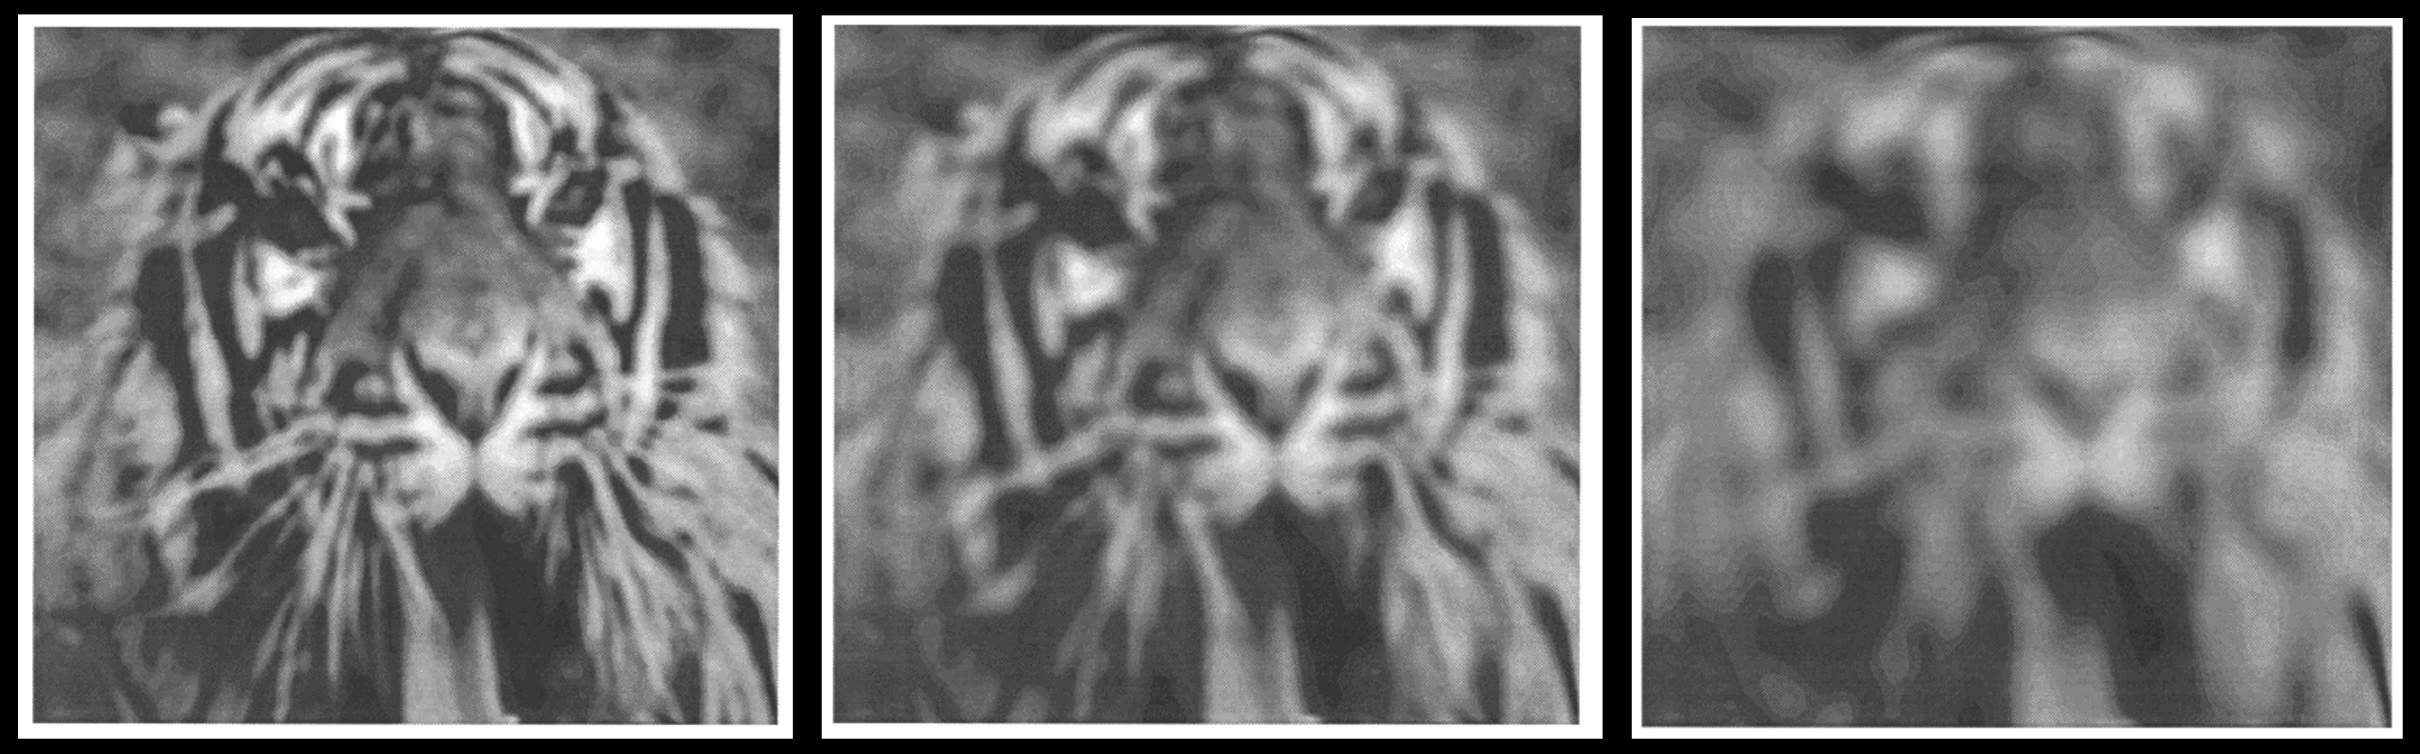
\includegraphics[width=0.8\textwidth]{image-processing/effect-sigma.png}
    \caption{Effect of the standard deviation $\sigma$ on the image.\\ The parameter $\sigma$ is increased from left to right.}
\end{figure}

The combination of 2 Gaussian filters is a Gaussian filter:
\begin{equation*}
    G_{\sigma_1} * G_{\sigma_2} = G_{\sqrt{\sigma_1^2+\sigma_2^2}}
\end{equation*}

Each filter is separable, meaning that we can apply the filter in the $x$ direction and then in the $y$ direction:
\begin{equation*}
    G_\sigma*f = g_{\sigma\rightarrow}*g_{\sigma\uparrow}*f
\end{equation*}
This as a critical implication: filtering with a $n\times n$ Gaussian kernel can be implemented as two convolutions of size $n$, reducing the complexity from $O(n^2)$ to $O(n)$.

\paragraph*{Oriented Gaussian Filters}
By default, $G_\sigma$ smoothes the image by the same amount in all directions. This has the drawback of blurring edges in all directions, which might make edge detection harder later on in the image processing pipeline. If we have some information about preferred directions, we might want to smooth with some value $\sigma_1$ in the direction defined by the unit vector $\begin{bmatrix}a&b\end{bmatrix}$ and by $\sigma_2$ in the direction defined by $\begin{bmatrix}c&d\end{bmatrix}$. This can be achieved using:
\begin{equation*}
    G(x, y) = \frac{1}{C}\exp\left[-\frac{(ax+by)^2}{2\sigma_1^2}-\frac{(cx+dy)^2}{2\sigma_2^2}\right]
\end{equation*}
We can write this in a more compact form using the standard multivariate Gaussian notation:
\begin{equation*}
    G(x, y) = \frac{1}{C}\exp\left[-\frac{X^\tp\Sigma^-1 X}{2}\right] \quad\text{where}\quad X = \begin{bmatrix}
        x\\ y
    \end{bmatrix}
\end{equation*}
The two (orthogonal) directions of filtering are given by the eigenvectors of $\Sigma$, the amout of smoothing is given by the square root of the corresponding eigenvalues of $\Sigma$.

% Insert illustrations

\subsection{Image derivatives}
We will see in the next chapter a variety of techniques to solve the \emph{edge detection problem}. A building block of such methods are \emph{image derivatives}: intuitively, we want to be able to measure how much the contrast of the image change locally. Peaks in contrast variation can be somehow interpreted as being close to edges, since this would be the point where the contours of the object contrast with the background.
\subsubsection{Finite differences}

Therefore, we want to compute at each pixel $(x, y)$ the derivates. In the discrete case, we could take the difference between the left and right pixels:
\begin{equation*}
    \partfrac{I}{x} \simeq I[i+1, j] - I[i-1,j]
\end{equation*}
This is equivalent as convoluting the image by:
\begin{equation*}
    \partial_x = \begin{bmatrix}
        1&0&-1
    \end{bmatrix}
\end{equation*}
The problem of this method is that it increases noise. Consider a noise model in which the actual image $I$ can be decomposed as the sum of the true, noiseless, image $\hat{I}$, and a noise $n$, following for instance a normal distribution. When then have $I=\hat{I}+n$, and we obtain:
\begin{equation*}
    \underbrace{I[i+1,j]-I[i-1,j]}_{\text{Actual image values}}=\underbrace{\hat{I}[i+1,j]-\hat{I}[i-1,j]}_{\text{True difference}}+\underbrace{n_++n_-}_{\text{Noises}}
\end{equation*}
Where $n_+-n_-$ follows a normal distribution of larger variance, providing therefore more noise on the derivate image.

\subsubsection{Smooth derivatives}
A solution is to first smooth the image by a Gaussian $G_\sigma$, and \emph{then} take derivatives:
\begin{equation*}
    \partfrac{f}{x} \simeq \partfrac{G_\sigma*f}{x}
\end{equation*}
Applying the differentiation property of the convolution \eqref{eq:diff-conv}:
\begin{equation*}
    \partfrac{f}{x} \simeq \partfrac{G_\sigma}{x}*f
\end{equation*}
Therefore, taking the derivative in $x$ of the image can be done by applying a convolution with the derivative of a Gaussian:
\begin{equation*}
    \partfrac{G_\sigma}{x}=\frac{1}{C}\cdot x\exp\left[-\frac{x^2+y^2}{2\sigma^2}\right]
\end{equation*}
Another crucial property is that the Gaussian derivative is also separable, reducing drastically the computational cost.

% TODO: insert graph of 1D/2D derivative of Gaussian

Smoothing before the derivative improves the results by reducing the noise, but still blurs away the edge information. In practice, there is always a tradeoff to find between smoothing and good edge localization.

\subsubsection{Beyond smooth derivatives}
Other methods are sometimes used in practice to overcome the limitations detailled above. \emph{Directional derivatives} are the equivalent of directional smoothing; we output the following quantity
\begin{equation*}
    \cos\theta\partfrac{G_\sigma}{x}+\sin\theta\partfrac{G_\sigma}{y}
\end{equation*}
This allows to avoid the smoothing of the edges while keeping the differentiation in directions that matter.

Second-order methods can also prove effective. This is a non-separable method, approximated by a difference of Gaussians. The output of the convolution is the Laplacian of the image; zero-crossing correspond to edges:
\begin{equation*}
    \nabla^2G_\sigma(x,y) = \partfrac{^2G_\sigma(x,y)}{x^2} + \partfrac{^2G_\sigma(x,y)}{y^2}
\end{equation*}

\section{Edge detection}

\section{Radiometry and Color}

\section{Color perception and Two-view geometry}

\section{Epipolar Geometry and Binocular Stereopsis}

\section{Markov random fields}

\section{Recovering structure from motion}

\section{Mean-shift algorithm for segmentation}

\section{Multi-view object models}

\section{Neural Networks for Visual recognition}

\section{Learning methods}


\end{document}